\documentclass[oneside,11pt]{Latex/Classes/PhDthesisPSnPDF}

% This file contains macros that can be called up from connected TeX files
% It helps to summarise repeated code, e.g. figure insertion (see below).

% insert a centered figure with caption and description
% parameters 1:filename, 2:title, 3:description and label
\newcommand{\figuremacro}[3]{
	\begin{figure}[htbp]
		\centering
		\includegraphics[width=1\textwidth]{#1}
		\caption[#2]{\textbf{#2} - #3}
		\label{#1}
	\end{figure}
}

% insert a centered figure with caption and description AND WIDTH
% parameters 1:filename, 2:title, 3:description and label, 4: textwidth
% textwidth 1 means as text, 0.5 means half the width of the text
\newcommand{\figuremacroW}[4]{
	\begin{figure}[htbp]
		\centering
		\includegraphics[width=#4\textwidth]{#1}
		\caption[#2]{\textbf{#2} - #3}
		\label{#1}
	\end{figure}
}

% inserts a figure with wrapped around text; only suitable for NARROW figs
% o is for outside on a double paged document; others: l, r, i(inside)
% text and figure will each be half of the document width
% note: long captions often crash with adjacent content; take care
% in general: above 2 macro produce more reliable layout
\newcommand{\figuremacroN}[3]{
	\begin{wrapfigure}{o}{0.5\textwidth}
		\centering
		\includegraphics[width=0.48\textwidth]{#1}
		\caption[#2]{{\small\textbf{#2} - #3}}
		\label{#1}
	\end{wrapfigure}
}

% predefined commands by Harish
\newcommand{\PdfPsText}[2]{
  \ifpdf
     #1
  \else
     #2
  \fi
}

\newcommand{\IncludeGraphicsH}[3]{
  \PdfPsText{\includegraphics[height=#2]{#1}}{\includegraphics[bb = #3, height=#2]{#1}}
}

\newcommand{\IncludeGraphicsW}[3]{
  \PdfPsText{\includegraphics[width=#2]{#1}}{\includegraphics[bb = #3, width=#2]{#1}}
}

\newcommand{\InsertFig}[3]{
  \begin{figure}[!htbp]
    \begin{center}
      \leavevmode
      #1
      \caption{#2}
      \label{#3}
    \end{center}
  \end{figure}
}


%%% Local Variables: 
%%% mode: latex
%%% TeX-master: "~/Documents/LaTeX/CUEDThesisPSnPDF/thesis"
%%% End: 


\usepackage{subfig}
\usepackage{pdfpages}

\hbadness=10000
\hfuzz=50pt

\begin{document}

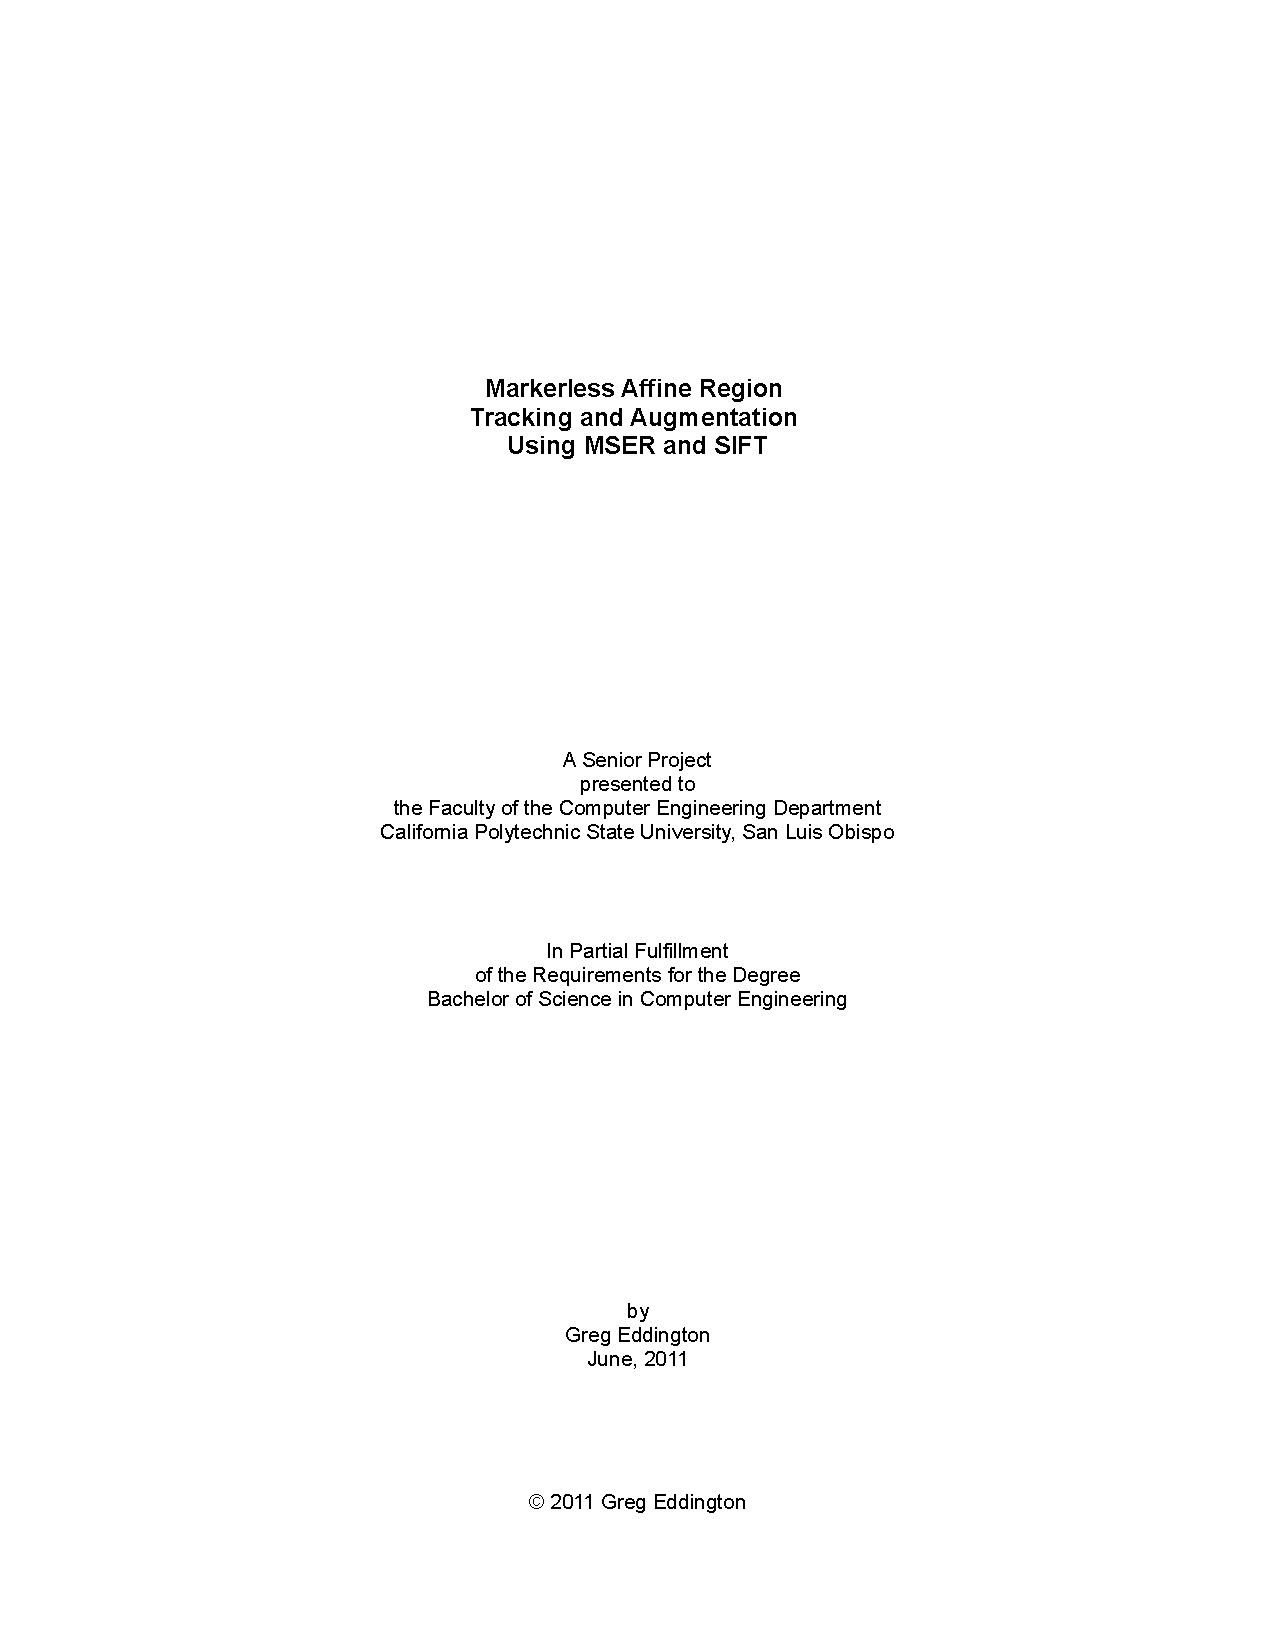
\includepdf{Cover/Markerless_Affine_Region_Tracking_and_Augmentation_Using_MSER_and_SIFT.pdf}

\renewcommand\baselinestretch{1.2}
\baselineskip=18pt plus1pt

\begin{abstracts}
Due to the advancements in mobile computing hardware and the inclusion of cameras in many computing platforms, augmented reality systems have become widely available.  This paper presents a real-time implementation of a novel markerless augmented reality algorithm which is able to track two-dimensional affine regions without a priori information of the environment or computing a world model.  The implementation consists of the MAR library; a modular software library which performs the region detection, identification, and tracking; and the Lighthouse application; a program which uses the MAR library to allow the user to augment scenes viewed from a camera.  The algorithm used in this paper is able to track textured affinely invariant planar regions using the maximally stable extremal region (MSER) detector to detect the regions and scale-invariant feature transform (SIFT) detector to identify the regions.  If three or more points from the region are matched across frames, an affine transformation is calculated which can be used to augment the scene by transforming a two-dimensional virtual image, causing it to appear to be stationary with respect to the region being tracked.  Testing found that the system is robust at tracking translation, scale, and rotational changes in regions at a frame-rate adequate for real-time applications and is able to handle changes in angle and illumination.   
\end{abstracts}

\frontmatter

%: ----------------------- Table of Contents ----------------------------------
\setcounter{secnumdepth}{3}
\setcounter{tocdepth}{3}
\tableofcontents

%: ----------------------- List of Figures and Tables -------------------------
\listoffigures
\listoftables

%: ---------------------- Main Document ---------------------------------------
\mainmatter

\chapter{Introduction}

Augmented reality (AR) is a field of computer vision which incorporates virtual images into real-world images.  An augmented reality system is designed to blend computer generated images into camera footage in real time.  AR has become increasingly popular in the field of mobile electronics, as the increase in power and the addition of high-resolution cameras have allowed for mobile augmented reality to become feasible in consumer electronics.  Wikitude is an example of a mobile augmented reality application, able to combine computer generated landmark information over a physical image of landmarks \cite{wikitude_11}.

\begin{figure}[h!]
  \center{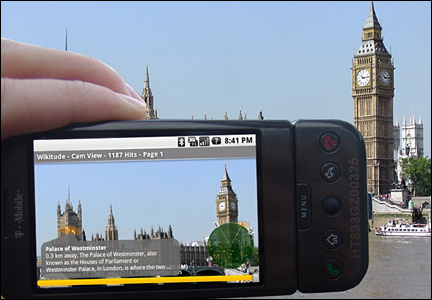
\includegraphics[width=0.5\textwidth]
        {Images/wikitude_example.png}}
  \caption{\label{fig_wikitude_example} An image from Wikitude, a mobile augmented reality application, augmenting a scene of a landmark with information about the landmark \cite{wikitude_11}.} 
\end{figure}

An augmented reality system is generally compromised of three core components: one or more cameras, a display, and a computer.  Most cameras can be used for augmented reality systems, although higher quality images are preferred as they allow for easier object recognition and tracking.  Three forms of displays are often used in AR systems.  Head mounted displays are worn over the users eyes and augment what the user sees.  A magic mirror setup involves a screen which is placed across from a user with a camera pointing at the user, creating an setup similar to a mirror which displays an augmented scene.  A magic lens setup uses a handheld screen with a camera mounted on the back, allowing the user to view "through" the device to see an augmented scene.  These three display styles are shown in figure \ref{fig_ar_displays}.  
 
\begin{figure}[h!]
  \centering
  \subfloat[Head Mounted Display \cite{marano_09}]{\label{fig_headmounted_display}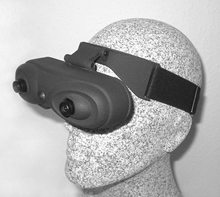
\includegraphics[width=0.33\textwidth]{Images/headmounted_display.png}}\quad\subfloat[Magic Mirror \cite{artag_09}]{\label{fig_magic_mirror}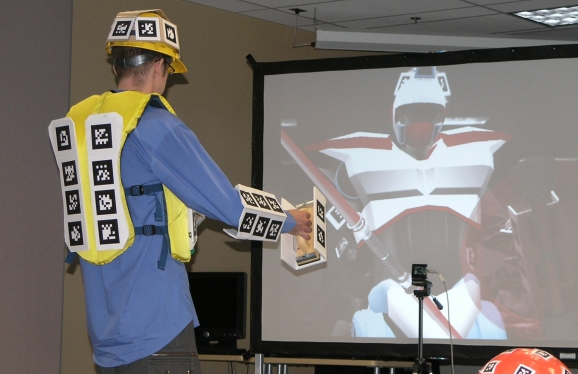
\includegraphics[width=0.33\textwidth]{Images/magic_mirror.png}}\quad\subfloat[Magic Lens \cite{layar_11}]{\label{fig_magic_lens}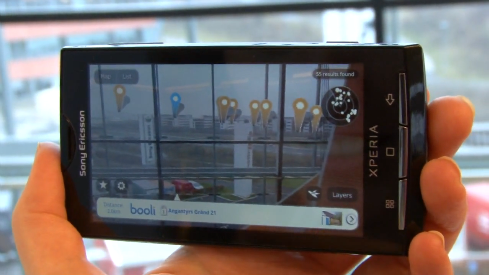
\includegraphics[width=0.33\textwidth]{Images/magic_lens.png}}
  \caption{\label{fig_ar_displays} Three common display setups used in augmented reality systems.} 
\end{figure}

\chapter{Background}

Several algorithms exist for augmenting reality.  Two key features which distinguish various augmented reality algorithms are whether or not they require a priori information and whether or not they require a world view.  A common characteristic of augmented reality systems which require a priori information is the use of markers.  The marker's appearance and dimensions are known by the AR system beforehand.  The algorithms are designed to look for that specific marker, and use the a priori information given about it to augment the scene with a virtual image.  Table \ref{table_characteristics} describes the advantages and disadvantages of using markers in an AR system.  When using markers in an AR system, the system knows which surfaces to augment via a priori information and regions are identified by matching them to known patterns.  When markers are not used in an AR system, the system learns which surfaces to augment via user input and regions are detected and tracked by looking for distinguishing keypoints.

\begin{table}[h]
\centering
\begin{tabular}{| p{2.5cm} | p{5.5cm} | p{5.5cm} |} 
\hline
{\bf Characteristic} & {\bf Advantages} & {\bf Disadvantages} \\ \hline

{\bf Markers} & Three dimensional information can be extracted knowing the dimensions of the marker. & Requires the user to add unnatural markers to the physical scene. \\
 & & \\
 & Markers can cue the system to augment the space differently based on physical patterns. & Markers may require extra work from the user to create. \\
 & & \\
 & & Only regions  where markers can be placed can be augmented. \\ \hline

{\bf Spatial Awareness} & Three dimensional information can be extracted knowing the location of the camera relative to the region. & Systems require additional sensors, such as gyroscopes and GPS sensors. \\
 & & \\
 & Markers can cue the system to augment the space differently based on spatial location. & Prohibits augmentation using existing cameras without position sensors, such as webcams. \\ \hline
\end{tabular}
\caption[Advantages and Disadvantages of AR Characteristics]{\textbf{Advantages and Disadvantages of AR Characteristics} - Advantages and disadvantages of common characteristics of augmented reality systems.}
\label{table_characteristics}
\end{table}

ARToolKit is an example of an AR system which makes use markers to allow virtual objects to be augmented into a scene (shown in figure \ref{fig_artoolkit_example}) \cite{kato_99}, while Golfscape is an example of an AR system which uses spatial awareness in order to augment the distance to various golf course features into a view of the course (shown in figure \ref{fig_golfscape_example}) \cite{golfscape_10}.  The algorithm described and implemented in this paper is built on work by Matt Marano in his thesis Affine Region Tracking and Augmentation Using MSER and Adaptive SIFT Model Generation \cite{marano_09}.  This approach does not use markers or spatial awareness to create an AR system, creating an algorithm flexible for many environments, requiring only a commodity camera with no additional hardware and no alterations to the scene which will be augmented.

\begin{figure}[h!]
  \center{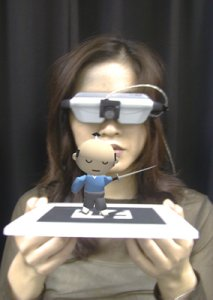
\includegraphics[width=0.5\textwidth]
        {Images/artoolkit_example.png}}
  \caption{\label{fig_artoolkit_example} An image from ARToolKit, an augmented reality library, augmenting a scene using markers physically placed into the environment \cite{artoolkit_11}.}
\end{figure}

\begin{figure}[h!]
  \center{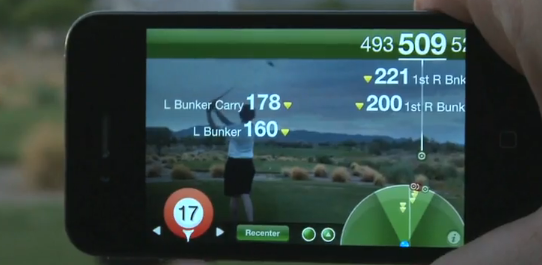
\includegraphics[width=0.5\textwidth]
        {Images/golfscape_example.png}}
  \caption{\label{fig_golfscape_example} An image from Golfscape, a mobile augmented reality application which uses a GPS and solid state compass to augment golf course information onto images of the course streamed from the phone's camera \cite{golfscape_10}.} 
\end{figure}

\section{Project Requirements}

The goal of this project is to implement a markerless augmented reality algorithm which can track and augment two-dimensional affine regions.  The following were the requirements the project aimed to fulfill:

\begin{description}
\item[Affine Region Detection] The ability to detect affine surfaces which can be used as surfaces for augmentation.
\item[Affine Region Tracking and Augmentation] The ability track a selected affine surface and calculate an affine transformation matrix which can transform any point on the surface from an initial camera frame to subsequent camera frames.
\item[No A Priori Information] The ability to augment a scene with no information given a priori, such as marker patterns.
\item[No World Model] The ability to augment a scene without using a world model to store the location of objects in the environment or the use of GPS or gyroscopic information. 
\item[Implementation] An implementation of this algorithm in C/C++ to allow for use on multiple platforms.
\item[Reusable Code] The creation of a software library which can be reused in future projects which wish to use this markerless augmentation algorithm.
\item[Real-Time Augmentation] The ability to augment reality in real time and not only in post-processing.
\item[Modular Camera Support] A modular design which can allow for the support of different types of camera hardware.
\item[Configurable Environment] A configurable design which allows for the augmentation to be fine-tuned to different environments and use cases.

\end{description}

\chapter{Design}

\section{Computer Vision Algorithms}

The design of the markerless augmented reality algorithm presented in this paper relies on a two phase approach.  The affine region detection phase involves using the maximally stable extremal regions (MSER) computer vision algorithm to detect affine regions in the camera frame.  The region tracking and affine transform calculation phase involves using the scale-invariant feature transform (SIFT) computer vision algorithm to track a chosen affine region and calculate a transform to map model space to camera space for the region, which can later be used for augmentation.

As the MSER and SIFT algorithms are key to the augmentated reality system, a brief description of both is provided.  A summary of the two computer vision algorithms is presented in table \ref{table_mser_and_sift}.

\subsection{Maximally Stable Extremal Region (MSER)}

The maximally stable extremal region (MSER) detector computer vision algorithm was created to establish correspondence between two images of a scene from different viewpoints \cite{matas_02}.  The detector finds regions of continuously connected pixel "blobs" which are both extremal and maximally stable.  The detector can be used to find affine regions.  These regions are robust to changes in viewpoint, rotation, scale, and lighting when compared to other affine region detectors \cite{mikolajczyk_05}.  While the MSER are blobs, they are often represented with an ellipse as shown in figure \ref{fig_mser_features}.

\begin{figure}[h!]
  \center{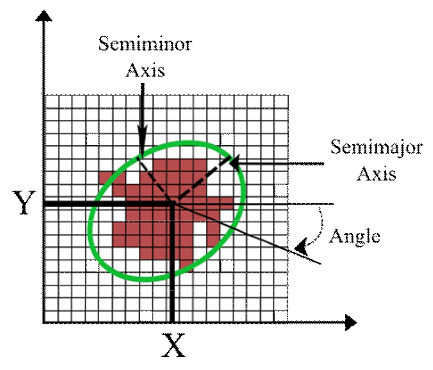
\includegraphics[width=0.6\textwidth]
        {Images/mser_features.png}}
  \caption{\label{fig_mser_features} The features which describe maximally stable extremal regions \cite{marano_09}.}
\end{figure}

\begin{figure}[h!]
  \center{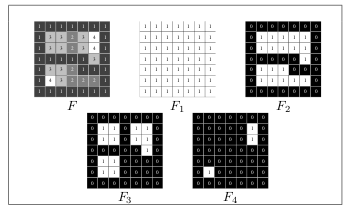
\includegraphics[width=0.8\textwidth]
        {Images/mser_sequence.png}}
  \caption{\label{fig_mser_sequence} The progression of thresholding performed in the MSER algorithm. \cite{najman_06}.}
\end{figure}

The MSERs of a frame are found by thresholding the gray-scale of the image at all possible thresholds.  This creates a sequence of images which begin as all white and gradually changes to an image of all black pixels, as shown in figure \ref{fig_mser_sequence}.  Maximal regions are the set of all connected regions of all frames.  Maximally stable regions are ones where the relative area change as a function of relative change of threshold is at a local minimum \cite{matas_02}.

\subsection{Scale-Invariant Feature Transform}

The scale-invariant feature transform (SIFT) detector is a computer vision algorithm which was created to find and describe local features in an image \cite{lowe_99}.  It finds keypoints in a camera frame that are affinely invariant to changes in translation, rotation, and scale.  These keypoints are represented as circular regions, shown in figure \ref{fig_sift_features}.

\begin{figure}[h!]
  \center{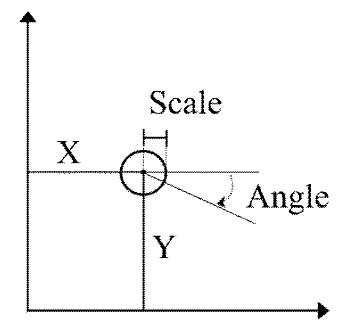
\includegraphics[width=0.5\textwidth]
        {Images/sift_features.png}}
  \caption{\label{fig_sift_features} The features which describe SIFT keypoints \cite{marano_09}.}
\end{figure}

The SIFT algorithm begins by identifying regions of interest.  It does this by Gaussian blurring the image at multiple levels in make the method invariant to scale.  It then performs a difference of Gaussians (DoG) by subtracting adjacent levels of the Gaussian blurred images in order to find stable regions, shown in figure \ref{fig_difference_of_gaussian}.  Regions of interest are found by locating the local maxima and minima in the image.  If a pixel is less than or greater than all 26 neighbors (the 8 surrounding it on the current scale, the 9 on the previous scale, and the 9 on the following scale, as shown in figure \ref{fig_nearest_neighbors}) it is considered a region of interest.

\begin{figure}[h!]
  \center{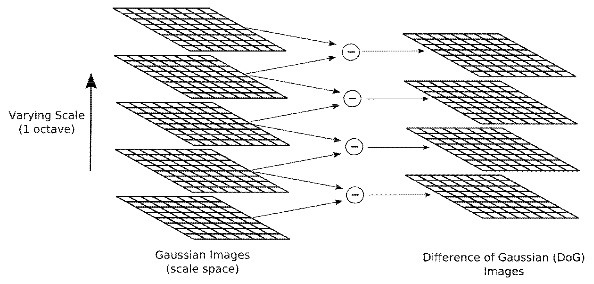
\includegraphics[width=\textwidth]
        {Images/difference_of_gaussian.png}}
  \caption{\label{fig_difference_of_gaussian} A difference of Gaussians is performed on several different levels of Gaussian blurring on an image in the SIFT filter \cite{marano_09}.}
\end{figure}

\begin{figure}[h!]
  \center{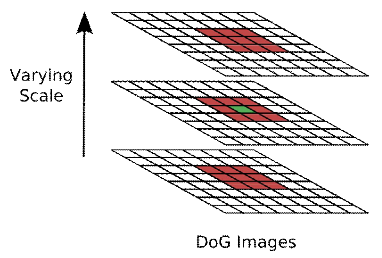
\includegraphics[width=0.6\textwidth]
        {Images/nearest_neighbors.png}}
  \caption{\label{fig_nearest_neighbors} The extrema are found by comparing a pixel with its 26 neighbors, with 9 being from the previous level of DoG and 9 being from the next level \cite{marano_09}.}
\end{figure}

The second phase of the SIFT algorithm filters out noisy points.  Noisy points are those with low contrast and those which are poorly localized.  Points with a low value in the difference of Gaussians function are considered to be low contrast and are filtered out, as shown in \ref{fig_sift_contrast}. 
Poorly localized points are detected by finding keypoints which have a large principle curvature perpendicular to an edge and a small principle curvature in the direction of the edge.  These points are filtered out as shown in figure \ref{fig_sift_localization}.

\begin{figure}[h!]
  \centering
  \subfloat[Local extrema found from the DoG of an image are considered regions of interest.]{\label{fig_sift_extrema}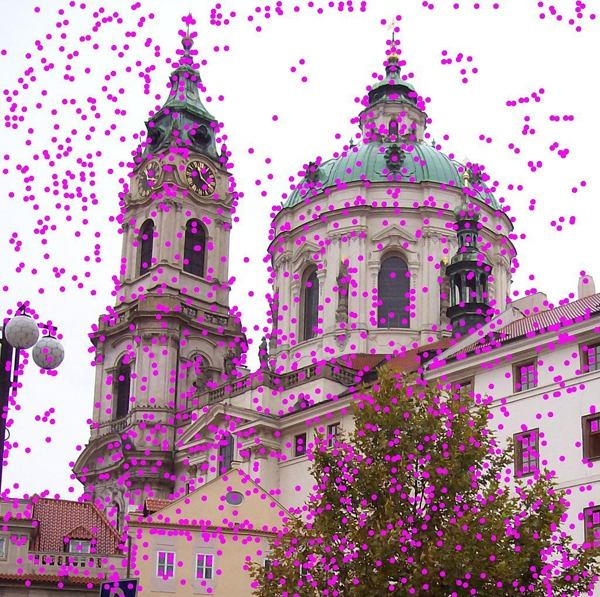
\includegraphics[width=0.45\textwidth]{Images/sift_extrema.png}}\quad\subfloat[Regions of interest with low contrast are filtered out.]{\label{fig_sift_contrast}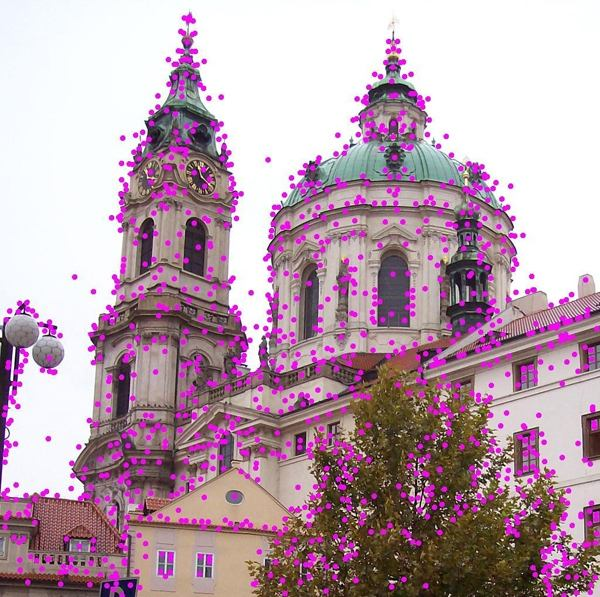
\includegraphics[width=0.45\textwidth]{Images/sift_contrast.png}}\quad\subfloat[Regions of interests with poor localization are filtered out, leaving the keypoints.]{\label{fig_sift_localization}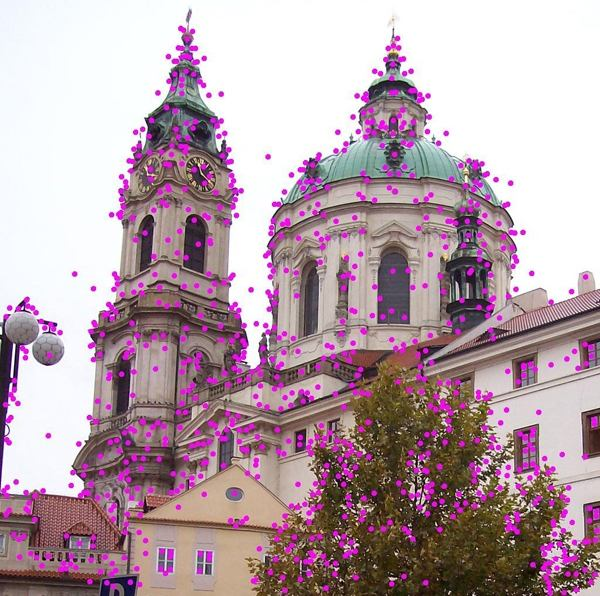
\includegraphics[width=0.45\textwidth]{Images/sift_localization.png}}
  \caption{\label{fig_sift_filtering} Regions of interest being filtered in the SIFT algorithm to the final keypoints.} 
\end{figure}

\begin{table}[h]
\centering
\begin{tabular}{| p{2cm} | p{5.75cm} | p{5.75cm} |} 
\hline
{\bf Name} & Maximally Stable Extremal Region (MSER) & Scale-Invariant Feature Transform (SIFT) \\ \hline
{\bf Regions} & Continuously connected pixel regions & Circular keypoint \\ \hline
{\bf Region Representation} & Ellipse & Circle \\ \hline
{\bf Detector Criteria} & Maximum or minimum image intensity relative to overall frame  & Maximum or minimum image intensity relative to local area \\ \hline
{\bf Region Description} & Center$_x$, Center$_y$, Variance$_x$, Variance$_y$, Mean & Center$_x$, Center$_y$, Scale, Angle, 128 Element Descriptor \\ \hline
\end{tabular}
\caption[Vision Detector Summary]{\textbf{Vision Detector Summary} - A summary of the MSER and SIFT detectors \cite{marano_09}.}
\label{table_mser_and_sift}
\end{table}

\section{Design Overview}

A diagram of the flow of the algorithm is presented in Figure \ref{fig_mar_algorithm_flow}.  As mentioned before, the algorithm is divided into a affine region detection phase and a region tracking and transform calculation phase.  

\begin{figure}[h!]
  \center{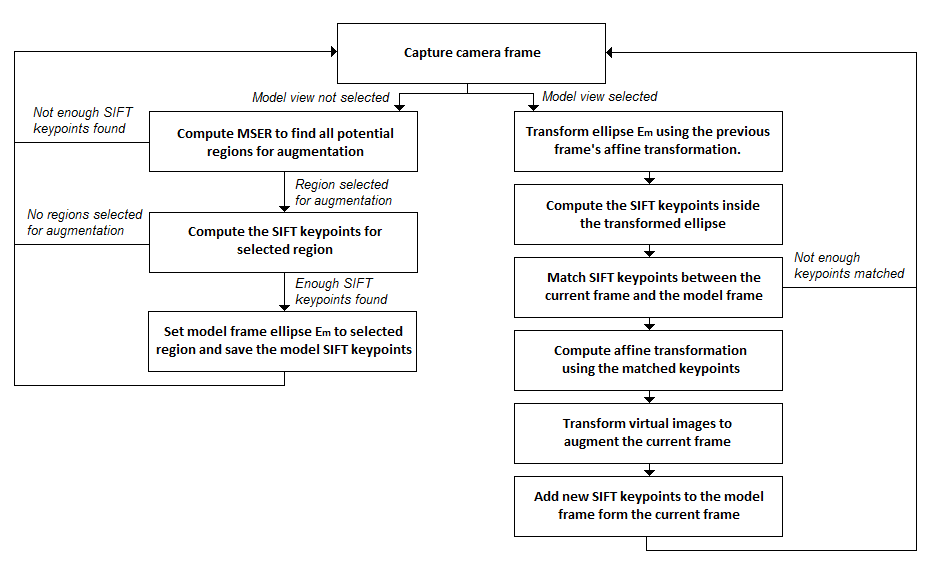
\includegraphics[width=\textwidth]
        {Images/mar_algorithm_flow.png}}
  \caption{\label{fig_mar_algorithm_flow} A flow diagram of the algorithm presented in this paper.}
\end{figure}

\section{Affine Region Detection}

The algorithm will identify potential candidates for augmentation by calculating the MSER in a camera frame.  An example of the MSER detected in a camera frame is shown in figure \ref{fig_mser_example}.  The user can select one of these regions for augmentation.  The MSER is then used to determine the region to augment.

\begin{figure}[h!]
  \center{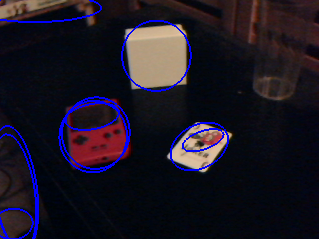
\includegraphics[width=0.5\textwidth]
        {Images/mser_example.png}}
  \caption{\label{fig_mser_example} An example of several ellipse representing MSER found in a camera frame.  These are potential candidates for augmentation.}
\end{figure}

The SIFT algorithm is then used to identify all keypoints within the frame.  The SIFT keypoints within the selected MSER are recorded as the model keypoints and the selected MSER ellipse is recorded as the model ellipse.  A visual representation of SIFT keypoints found in a camera frame is shown in figure \ref{fig_sift_example}.

\begin{figure}[h!]
  \center{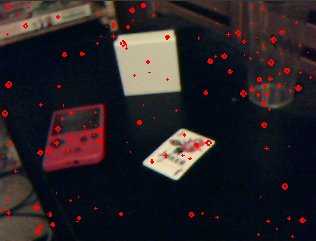
\includegraphics[width=0.5\textwidth]
        {Images/sift_example.png}}
  \caption{\label{fig_sift_example} An example of several SIFT keypoints found in a camera frame.  These are used for region identification and tracking.}
\end{figure}

\section{Affine Region Tracking}

Once an affine region has been selected and the model view frame has been recorded, the region is tracked in subsequent frames.  The model view ellipse is transformed using the previous frame's affine transformation in order to transform the ellipse into the last frame's space.  This transforms the search space into the region of the last frame.  The SIFT keypoints within the transformed ellipse are then matched with SIFT keypoints in the model view ellipse.  Assuming camera space does not change much between frames, limiting keypoints to the ellipse of the last frame can help reduce matching keypoints with different but similar appearing targets in the frame.  This also reduces the search space the SIFT algorithm needs to cover per frame.  As a backup, if the region cannot be matched within the search space of the ellipse transformed with the previous frame's affine transformation, the whole camera frame is then used as a search space for the SIFT algorithm.

In order to match SIFT keypoints between the model view and the current camera view, the distance between all keypoints in the model view and all keypoints in the current camera view is calculated using \ref{eq_keypoint_distance}, where $k_1$ and $k_2$ are keypoints.  The keypoint with the lowest distance is chosen as the best match, but in order to prevent matching between ambiguous or dissimilar keypoints, \ref{eq_keypoint_unambiguous} and \ref{eq_keypoint_matched} are used to check if the match is valid. $\sigma$ controls how unambiguous the matching must be, and $\delta_{max}$ controls the maximum distance threshold for a pair of keypoints to be considered matching.

\begin{equation} 
\label{eq_keypoint_distance}
distance = \displaystyle\sum\limits_{i=0}^{128} |k_1 descriptor_i - k_2 descriptor_i|
\end{equation}

\begin{equation} 
\label{eq_keypoint_unambiguous}
distance_{best} * \sigma < distance_{second best}
\end{equation}

\begin{equation} 
\label{eq_keypoint_matched}
distance_{best} < \delta_{max}
\end{equation}

A minimum number of matching keypoints, greater than 3, can be defined as a threshold to consider a region matched between the model frame and current camera frame.  If at least this many keypoints are matched, then the algorithm proceeds to calculate the affine transform, otherwise it proceeds to the next frame without augmenting the scene.

\section{Affine Transformation Calculation}

After finding matching keypoints between the model view frame and the current frame, the affine transformation is calculated which can be used to augment the scene.  An affine transformation can be calculated from the model view frame to the current frame using three or more distinct points.  

An affine transformation will map a point (x, y) to a transformed point (u, v) using translation, rotation, and scaling.  The affine transformation can be written as a matrix product of a 3x3 affine transformation matrix as shown in \ref{eq_affine_transform}, where $m_{1}$-$m_{4}$ are rotational and scaling values and $t_x$ and $t_y$ are translation values.

\begin{equation} 
\label{eq_affine_transform}
\left[
  \begin{array}{ c }
     u \\
     v \\
     1
  \end{array} 
\right]
=
\left[
  \begin{array}{ c c c }
     m_1 & m_2 & t_x \\
     m_3 & m_4 & t_y \\
     0 & 0 & 1
  \end{array} 
\right]
\left[
  \begin{array}{ c }
     x \\
     y \\
     1
  \end{array} 
\right]
\end{equation}

Given at least three matching points from the model-view frame ($x_n$, $y_n$) and the current frame ($u_n$, $v_n$), the unknowns $m_{1}$-$m_{4}$, $t_x$, and $t_y$ can be solved in \ref{eq_affine_transform} using \ref{eq_affine_solve} \cite{marano_09}.

\begin{equation} 
\label{eq_affine_solve}
\left[
  \begin{array}{ c c c c c c }
     x_1 & y_1 & 0 & 0 & 1 & 0 \\
     0 & 0 & x_1 & y_1 & 0 & 1 \\
     x_2 & y_2 & 0 & 0 & 1 & 0 \\
     0 & 0 & x_2 & y_2 & 0 & 1 \\
     & & & ... & & \\
     & & & ... & & \\
     x_n & y_n & 0 & 0 & 1 & 0 \\
     0 & 0 & x_n & y_n & 0 & 1
  \end{array} 
\right]
\left[
  \begin{array}{ c }
     m_1 \\
     m_2 \\
     m_3 \\
     m_4 \\
     t_x \\
     t_y
  \end{array} 
\right]
=
\left[
  \begin{array}{ c }
     u_1 \\
     v_1 \\
     u_2 \\
     v_2 \\
     ... \\
     ... \\
     u_n \\
     v_n
  \end{array} 
\right]
\end{equation}

\section{Augmentation}

Using the affine transformation, the scene can be augmented with a virtual image.  Because the affine transformation is able to transform any point on the affine surface from model view space to the space in the current camera frame, a virtual image can be drawn into the frame to appear as if it is part of the affine surface.  Points which compose a virtual image in the initial model view frame are transformed using the affine transformation and drawn in subsequent frames to augment reality. 

\section{Updating Model View Frame}

In order account for gradual changes in the region being tracked, new keypoints are added to the model space and old keypoints are removed from the model space.  This can allow the system to have more robust affine region tracking through gradual changes in scene, such as a gradual change in lighting or camera focus.  Adding keypoints can also help reduce the effect of noise in the SIFT filter which can cause keypoints to not appear during the frame when the model view was initially recorded.

In order to gradually add new keypoints, after an affine transformation is successfully computed, the model view MSER ellipse is transformed to the space of the current frame.  All SIFT keypoints within the ellipse are recorded.  In order to reduce the chance of adding keypoints which aren't part of the affine region (for example, if a mismatch occurs between SIFT keypoints and the affine transform is not valid), a keypoint is required to appear in the transformed ellipse in a paramerizable number of consecutive frames.  Once a keypoint has appeared in the specified number of frames, it is transformed into model space from the current camera frame's space using the inverse of the affine transformation.  Old keypoints can be removed when adding new keypoints using various priorities, such as least recently used or round robin.

\chapter{Implementation}

The markerless affine region tracking augmented reality algorithm presented in this paper was implemented in two components: the Markerless Augmented Reality (MAR) library and the Lighthouse application.  These two programs are described in table \ref{table_code_summary}

\begin{table}[h]
\centering
\begin{tabular}{| l | l | l | p{6.5cm} |} 
\hline
{\bf Name} & {\bf Type} & {\bf Language(s)} & {\bf Summary} \\ \hline
MAR & Library & C and C++ & Contains camera interfacing code, computer vision 
algorithms, and the augmented reality computations \\ \hline
Lighthouse & Application & C & An example and test application which uses the MAR library.  It contains code to display the augmented scene and handle user input. \\ \hline
\end{tabular}
\caption[Summary of Code]{\textbf{Summary of Code} - Summary of the pieces of code which make up the augmented reality implementation.}
\label{table_code_summary}
\end{table}

\section{MAR Library}

The MAR library contains the camera interfacing code, computer vision algorithms, and code which computes affine transformations.  It is the portion of software that user can use to add the capability to augment reality to their applications.

\subsection{Camera Interface}

The hardware interface to the camera is incorporated into the MAR library.  The camera interface is modular so that new camera support can be added to the MAR library.  This design approach was chosen to allow for simpler use of the library as users would not have to interface with the camera directly and to allow code written for using a specific camera in order to aid in augmenting reality to be incorporated into the library once and not be reproduced multiple times for different projects.

At the time of writing this paper, the MAR library currently supports Video4Linux2 cameras using memory mapping and a YUYV pixel format.  The library has been tested with a Logitech Webcam C160, which is the camera used in all images in this paper.

\subsection{Computer Vision}

The maximally stable extremal region (MSER) and scale-invariant feature transform (SIFT) computer vision algorithms were added to the MAR library from the VLFeat library.  The VLFeat library includes an implementation of both the MSER and SIFT algorithms designed for efficiency and compatibility \cite{vlfeat_08}.  This library is wrapped in the MAR library to abstract away unnecessary information from the VLFeat algorithm and create data structures which encapsulate data needed by the MAR library.

\subsection{Library Interface}

The MAR library contains two key interfaces necessary for utilization: the API and the configuration file.

\subsubsection{Application Programming Interface}

The MAR library API is designed with simplicity in mind, requiring a minimal amount of calls to successfully augment a scene, but providing a larger array of optional calls to fine tune augmentation.  The flow of function calls to use the MAR library is outlined in figure \ref{fig_mar_api_calls}.  The API is designed to use keys to identify library objects in function calls and have all function calls which can fail return an error code to signal whether or not they were successful and, if they failed, the reason why.

\begin{figure}[h!]
  \center{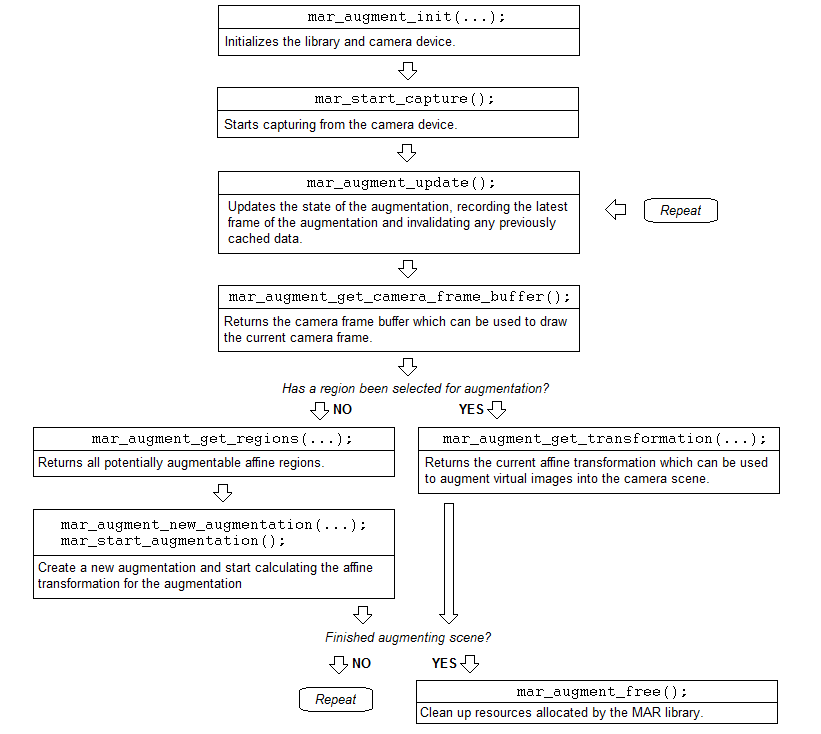
\includegraphics[width=\textwidth]
        {Images/mar_api_calls.png}}
  \caption{\label{fig_mar_api_calls} A flow diagram of the minimal API calls needed to use the MAR library.}
\end{figure}

\subsubsection{Configuration File}

The configuration file is used to parameterize many of the variables in the MSER, SIFT, and MAR algorithms.  The configuration file is also the location where the camera module is configured by the user.  A configuration file was incorporated into the library because it provided a simple interface for setting up the AR and camera environment across multiple programs.  Having a single unified configuration file format also allows for the possibility of using a calibration program to calibrate an environment for multiple programs which use the library.

The libconfig library was chosen to manage loading the configuration file as it provided a compact and readable file format which could be edited via a text editor \cite{libconfig_11}.  Parameters which are configured via the configuration file can also be configured in software via the MAR library API.

\section{Lighthouse Application}

Lighthouse is an example application which uses the MAR library.  It was designed to be used as an application to demonstrate the functionality of the MAR library and to test users' configurations.  It was also written to be used as a template for creating applications which use the MAR library.

Initially, Lighthouse presents the user with areas which are potential candidates for augmentation.  The user may then select an affine surface to augment using the mouse.  A virtual image will be placed onto the surface coplanar to the viewing plane.  The program then calls the update function from the MAR library to compute affine transformations for subsequent frames.  This affine transformation is used to augment the subsequent camera frames with the virtual image.  An example of a normal usage of the Lighthouse application is presented in figure \ref{fig_lighthouse_example}.

\begin{figure}[h!]
  \centering
  \subfloat[Green points displayed in the frame mark regions which are potential candidates for augmentation.]{\label{fig_lighthouse_augmentable_regions}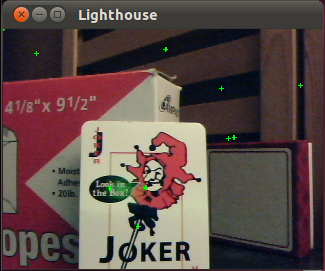
\includegraphics[width=0.4\textwidth]{Images/lighthouse_augmentable_regions.png}}\quad\subfloat[The user selects a playing card as the affine region to augment.]{\label{fig_lighthouse_selecting_region}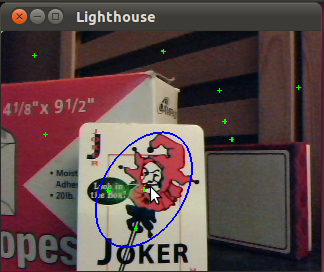
\includegraphics[width=0.4\textwidth]{Images/lighthouse_selecting_region.png}}
  \quad
  \subfloat[A virtual, four-colored squared is augmented into the scene in the initial frame.]{\label{fig_lighthouse_initial_frame}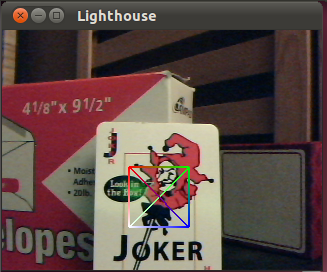
\includegraphics[width=0.4\textwidth]{Images/lighthouse_initial_frame.png}}\quad\subfloat[Using the MAR library, the affine region is tracked and the virtual image is augmented into subsequent frames.]{\label{fig_lighthouse_augmenting_reality}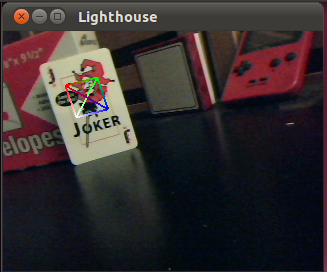
\includegraphics[width=0.4\textwidth]{Images/lighthouse_augmenting_reality.png}}
  \caption{Example usage of the Lighthouse application.}
  \label{fig_lighthouse_example}
\end{figure}

The Lighthouse application also allows users to configure the MAR library computer vision algorithm parameters.  This allows users to fine tune the augmented reality system to work better with their specific environment and desired use case.  An example of a user configuring the MSER and SIFT parameters is shown in figure \ref{fig_lighthouse_configure}.

\begin{figure}[h!]
  \centering
  \subfloat[A user configuring parameters for the MSER computer vision algorithm.]{\label{fig_lighthouse_configure_mser}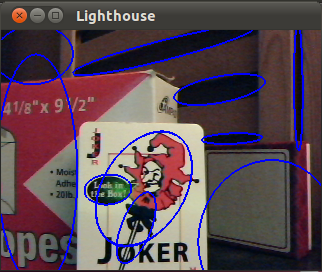
\includegraphics[width=0.4\textwidth]{Images/lighthouse_configure_mser.png}}\quad\subfloat[A user configuring parameters for the SIFT computer vision algorithm.]{\label{fig_lighthouse_configure_sift}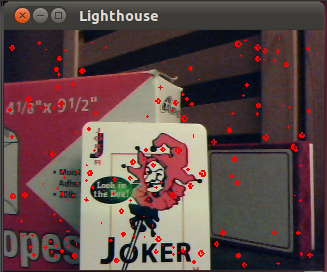
\includegraphics[width=0.4\textwidth]{Images/lighthouse_configure_sift.png}}
  \caption{Using Lighthouse to configure computer vision parameters for the augmentation algorithm.}
  \label{fig_lighthouse_configure}
\end{figure}

\chapter{Results}

All results were gathered running the Lighthouse application using the MAR library on a 2.2GHz Intel Celeron 900 processor running Ubuntu 11.04 using the 2.6.38 Linux kernel with a Logitech C160 webcam.

Several test cases were run to test various situations which would likely occur when augmenting a scene.  They are outlined in table \ref{table_test_cases}.  The scene being augmented is shown in figure \ref{fig_test_scene} and was chosen due to the fact it included multiple objects of different shapes in order to check that the algorithm could handle a busy scene.  The region being targeted for augmentation is the flat, green coupon booklet.  Images of the results are shown in figures \ref{fig_translation_augmentation}, \ref{fig_rotational_augmentation}, \ref{fig_scaling_augmentation}, \ref{fig_angle_augmentation}, and \ref{fig_obscured_augmentation}.  The tests scenes were augmented with a rate of 12 frames per second.

\begin{table}[h!]
\centering
\begin{tabular}{| c | c | p{8cm} |} 
\hline
{\bf Name} & {\bf Figure} & {\bf Description} \\ \hline
Translation & \ref{fig_translation_augmentation} & Tested the ability to augment the scene when the region being augmented is translated across the camera frame. \\ \hline
Rotation & \ref{fig_rotational_augmentation} & Tested the ability to augment the scene when the region being augmented is rotated within the camera frame. \\ \hline
Scaling & \ref{fig_scaling_augmentation} & Tested the ability to augment the scene when the region being augmented is moved towards and away from the camera lens. \\ \hline
Angle & \ref{fig_angle_augmentation} & Tested the ability to augment the scene when the angle between the camera and the region being augmented is increased. \\ \hline
Obscured & \ref{fig_obscured_augmentation} & Tested the ability to augment the scene when the region being tracked is obscured. \\ \hline
\end{tabular}
\caption[Test Cases]{\textbf{Test Cases} - A list and description of the various test cases performed using Lighthouse.}
\label{table_test_cases}
\end{table}

\begin{figure}[h!]
  \center{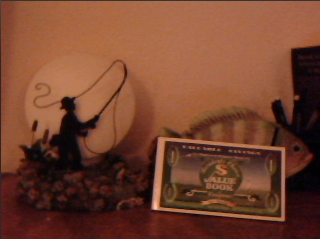
\includegraphics[width=\textwidth]
        {Images/test_scene.png}}
  \caption{\label{fig_test_scene} A scene used to test the MAR library.  The region being targeted for augmentation is a green coupon book.}
\end{figure}

For a affine region with distinguishable features, the MAR library performs well when augmenting a scene.  For translational and rotational changes the algorithm was able to augment all frames.  When changes in the scale of the region being augmented occurred, for the majority of the frames were able to be augmented.  The ability to augment the scene decreased as the region being augmented became smaller, causing the features of the region to be indistinguishable and unrecognizable.  This effect decreased when the change in size is gradual, as new keypoints are added for the smaller resolution region.  Augmentation often failed when moving the camera quickly, as the film time of the camera would cause a blurred frame from which the region being augmented was unable to be identified or tracked.  An example of this is shown in figure \ref{fig_blurred_augmentation}.

An additional test case was created to verify that only a recognizable portion of the region being augmented needs to be visible in order to augment the scene.  This test demonstrated that the algorithm requires only a portion of the region with at least 3 matching SIFT keypoints needs to be visible in order to be augmented successfully.

\begin{figure}[h!]
  \center{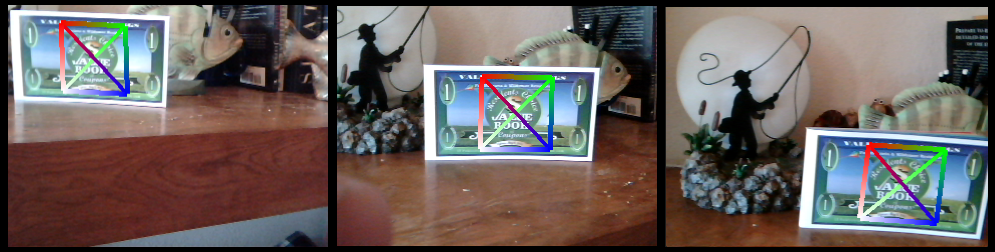
\includegraphics[width=\textwidth]
        {Images/translation_augmentation.png}}
  \caption{\label{fig_translation_augmentation} A virtual, four-colored square is augmented into the scene with a camera moving across the augmented region.}
\end{figure}

\begin{figure}[h!]
  \center{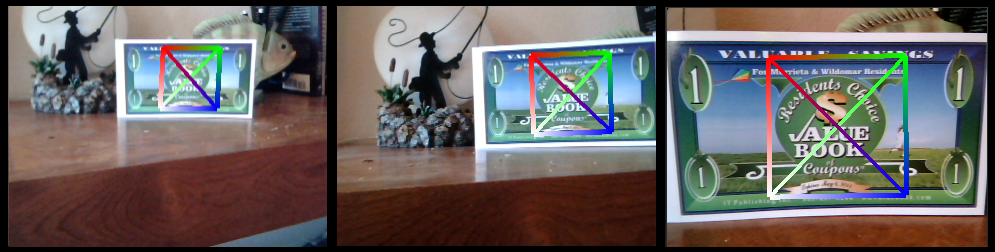
\includegraphics[width=\textwidth]
        {Images/scaling_augmentation.png}}
  \caption{\label{fig_scaling_augmentation} A virtual, four-colored square is augmented into the scene with a camera moving away and towards the augmented region.}
\end{figure}

\begin{figure}[h!]
  \center{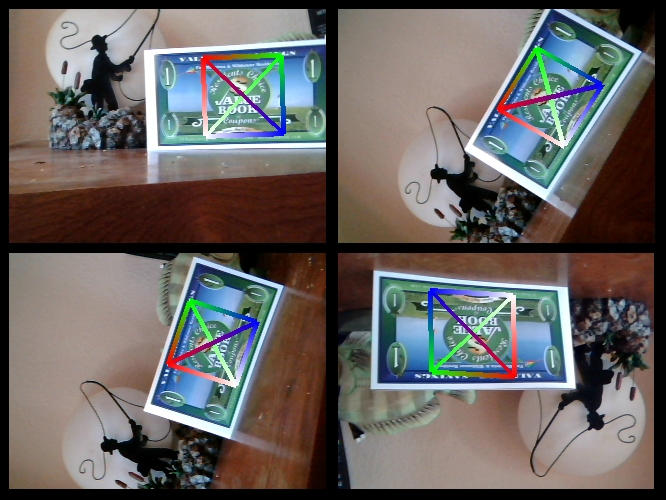
\includegraphics[width=\textwidth]
        {Images/rotational_augmentation.png}}
  \caption{\label{fig_rotational_augmentation} A virtual, four-colored square is augmented into the scene with a rotating camera.}
\end{figure}

\begin{figure}[h!]
  \center{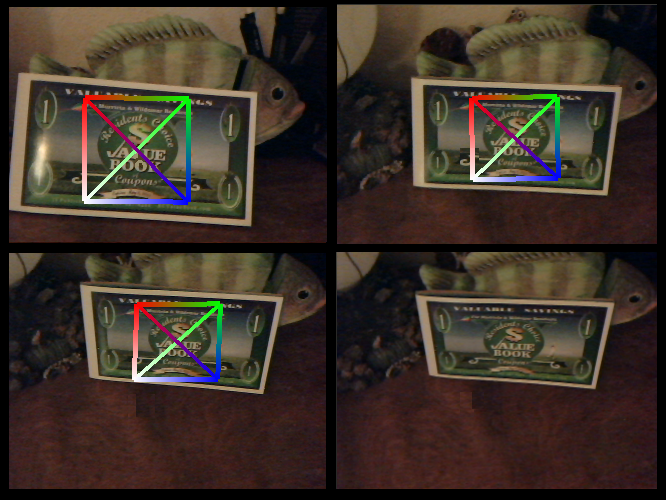
\includegraphics[width=\textwidth]
        {Images/angle_augmentation.png}}
  \caption{\label{fig_angle_augmentation} A virtual, four-colored square is augmented into the scene with the angle the augmented region is being viewed at increasing. At the last frame, the algorithm is unable to augment the region.}
\end{figure}

\begin{figure}[h!]
  \center{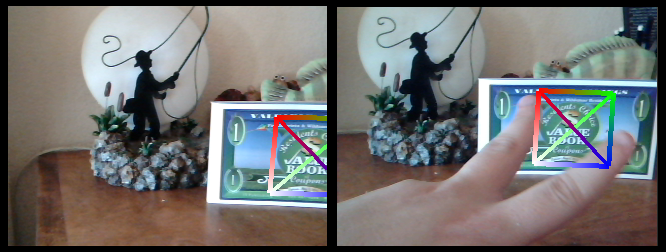
\includegraphics[width=\textwidth]
        {Images/obscured_augmentation.png}}
  \caption{\label{fig_obscured_augmentation} A virtual, four-colored square is augmented into the scene with the augmented region being partially obscured.}
\end{figure}

\begin{figure}[h!]
  \center{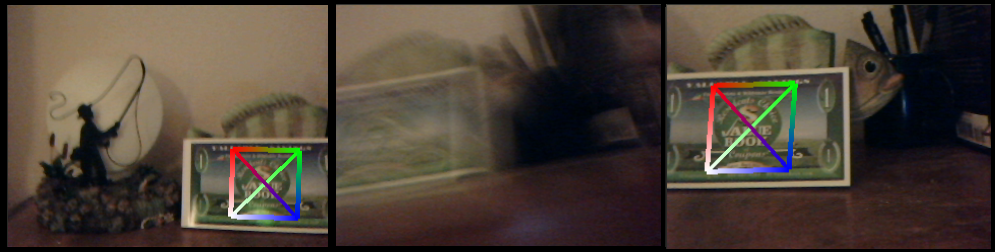
\includegraphics[width=\textwidth]
        {Images/blurred_augmentation.png}}
  \caption{\label{fig_blurred_augmentation} A virtual, four-colored square is augmented into the scene with a moving camera.  When the camera moves fast and creates a blurred image, the implementation is unable to augment the scene as shown in the middle frame.}
\end{figure}

\chapter{Conclusion}

The augmented reality system presented in this paper successfully augments scenes in many different environments.  The algorithms is robust at augmenting regions when the region varies in translation, rotation, and scale.  The algorithm is also successful at augmenting regions which are partially obscured as long as a sufficient number of SIFT keypoints are matched between the model view frame and the current frame.  The algorithm is most sensitive to blurring and changes in illumination, which cause SIFT keypoints from the model view frame to differ greatly from the current frame and prevent matching.  The system is also sensitive to changes in angle, as perspective effects become noticeable and negate the assumptions made about the ability to ignore the effect of perspective on the affine region.  

The algorithm was successfully implemented in C and C++ with the Markerless Augmented Reality (MAR) library and Lighthouse application.  The MAR library was created with the ability to be reused in multiple augmented reality projects with a modular design and simple interface.  The implementation supported real-time augmentation at an average frame rate of 12 frames per second on a 2.2GHz Intel Celeron 900 processor running Ubuntu 11.04 using the 2.6.38 Linux kernel with a Logitech C160 webcam.  The library was successfully designed to have the ability to support multiple cameras and have an interface for configuring the AR environment.

%------------------------ Appendix -------------------------------------------

\appendix

\chapter{Resources and Examples}

The MAR library and Lighthouse are released under the GPLv3 license.  Project source code, documentation, and video examples of Lighthouse running can be found at \url{http://code.google.com/p/mar-library/}.

% ----------------------- References -----------------------------------------
\pagebreak
\begin{footnotesize}
\bibliographystyle{Latex/Classes/PhDbiblio-url2}
\renewcommand{\bibname}{References}
\bibliography{references}
\end{footnotesize}

\end{document}
